% ============================================================
% ACL Findings Format — Multi-Lens Forensic Audit of AI Text Detectors
% Requires: acl2023.sty (available from ACL Rolling Review)
% Compile with: pdflatex → bibtex → pdflatex × 2
% ============================================================
\documentclass[11pt]{article}

% ---- Use the standard ACL style ----
% Download acl2023.sty from https://github.com/acl-org/acl-style-files
% If not available, this will still compile with a basic article class
\usepackage[hyperref]{acl2023}
\usepackage{times}
\usepackage{latexsym}
\usepackage{amsmath,amssymb}
\usepackage{booktabs}
\usepackage{graphicx}
\usepackage{subcaption}
\usepackage{xcolor}

\title{Audit of AI Text Detectors \\Under Editing-Depth Variation}

\author{
  Sid \\
  Manipal Institute of Technology \\
  Manipal, India \\
}

\begin{document}
\maketitle

\begin{abstract}
We present an audit of AI text detectors using topic-controlled paired evaluation across an editing-depth spectrum. Our Human Revision Study (HRS) comprises four domain-specific document pairs where all documents are AI-generated but differ in the degree of subsequent human editing. We audit a fine-tuned DeBERTaV3 classifier (AUROC $0.971$) and an SBERT baseline (AUROC $0.815$) through six complementary metrics: detector probability delta, $H_1$ topological density, Hypothesis Revision Index, cross-document BERTScore, and intra-document similarity. DeBERTa achieves near-maximal separation on all three high-intervention pairs ($\Delta \in [-0.982, -0.906]$). A zero-intervention anchor pair correctly yields $\Delta \approx 0$. Topological features do not reach significance ($p = 0.433$, $N = 3$). We contribute an experimental design and audit framework for studying how editing depth affects detector response.
\end{abstract}

\section{Introduction}

The evaluation of AI text detectors typically compares texts from \emph{different} topics, conflating topical signals with stylistic features~\cite{wang2024m4}. We introduce two contributions: (1)~a topic-controlled evaluation protocol (HRS) with four same-topic document pairs spanning an editing-depth spectrum; (2)~an audit framework combining six complementary metrics to study how the degree of human editing affects detector response.

\section{Related Work}

\paragraph{Neural \& Zero-Shot Detection.}
DetectGPT~\cite{mitchell2023detectgpt} uses log-probability curvature; Binoculars~\cite{hans2024binoculars} contrasts two LLMs ($>90\%$ at $0.01\%$ FPR); RAIDAR~\cite{mao2024raidar} measures rewriting edit distance. M4~\cite{wang2024m4} benchmarks multi-generator, multi-domain detection.

\paragraph{Topological Approaches.}
Tulchinskii et al.~\cite{tulchinskii2024intrinsic} show intrinsic dimensionality (PHD) separates human from AI text across 10 languages. Kushnareva et al.~\cite{kushnareva2023artificial} apply TDA to attention maps. Wei et al.~\cite{wei2025shortphd} extend PHD to short texts. Our $H_1$ density analysis on paired documents is exploratory and does not reach significance.

\paragraph{Adversarial Robustness.}
Krishna et al.~\cite{krishna2024paraphrasing} and Sadasivan et al.~\cite{sadasivan2023reliable,sadasivan2025adversarial} demonstrate detectors' vulnerability to paraphrasing. We do not evaluate adversarial robustness---a limitation we acknowledge.

\section{Methodology}

\subsection{Data}

\paragraph{AIHTD Corpus.} $N = 8{,}238$ labeled texts (80/20 stratified split).

\paragraph{HRS Pairs.} Four domain pairs (Table~\ref{tab:pairs}): three high-intervention (heavy human editing of AI-generated base text) and one zero-intervention anchor (no editing).

\begin{table}[t]
\centering
\small
\caption{HRS document pairs. HI = High-Intervention, ZI = Zero-Intervention.}
\label{tab:pairs}
\begin{tabular}{@{}llcc@{}}
\toprule
\textbf{Domain} & \textbf{Type} & \textbf{Base} & \textbf{Edited} \\
\midrule
Education      & HI   & 1{,}574 & 1{,}488 \\
Policy         & HI   & 1{,}956 & 1{,}966 \\
Sustainability & HI   & 324     & 355     \\
Sign/ISL       & ZI   & 6{,}199 & 5{,}917 \\
\bottomrule
\end{tabular}
\end{table}

\subsection{Detectors}

\paragraph{DeBERTaV3-Base.} Fine-tuned with split learning rates (backbone $2{\times}10^{-5}$, head $1{\times}10^{-4}$). Initial training failed (AUROC $0.50$, frozen classification head); repaired via gradient monitoring and Float32 inference:
\begin{equation}
    P_{\text{AI}}(x) = \text{softmax}\!\big(f_\theta(x)\big)_1
\end{equation}
where $f_\theta(x) \in \mathbb{R}^2$ are the classifier logits and subscript $1$ selects the AI-class probability.

\paragraph{SBERT Baseline.} Logistic regression on mean-pooled sentence-BERT embeddings (all-mpnet-base-v2).

\subsection{Evaluation Metrics}

For each HRS pair, we compute the \textbf{detector delta}:
\begin{equation}
    \Delta_d = P_{\text{AI}}^d(x_{\text{base}}) - P_{\text{AI}}^d(x_{\text{edited}})
\end{equation}

The \textbf{$H_1$ density} captures persistent 1-dimensional loops in sentence embedding point clouds $\mathcal{P} = \{e_1, \ldots, e_n\} \subset \mathbb{R}^{768}$:
\begin{equation}
    \rho_{H_1}(x) = \frac{\sum_{(b_i, d_i) \in \text{Dgm}_1(\mathcal{P})} (d_i - b_i)}{n}
\end{equation}
where $(b_i, d_i)$ are birth/death times from the Vietoris--Rips filtration ($\epsilon_{\max} = 2.0$) and $n$ is the sentence count.

The \textbf{HRI rate} is discourse marker density per 100 words; \textbf{Cross BERTScore} $F_1$ measures paired semantic overlap; \textbf{Intra-doc similarity} is mean pairwise cosine similarity among sentence embeddings.

\subsection{Statistics}

Paired permutation tests ($K = 1{,}000$) with Cohen's $d$:
\begin{equation}
    d = \frac{\bar{\Delta}}{s_{\Delta}}, \quad s_{\Delta} = \sqrt{\frac{1}{N-1}\sum_i (\Delta_i - \bar{\Delta})^2}
\end{equation}

\section{Results}

\subsection{AIHTD Performance}

DeBERTa: AUROC $= 0.971$. SBERT: AUROC $= 0.815$.

\subsection{HRS Audit}

\begin{table}[t]
\centering
\small
\caption{HRS multi-lens results. Bold: $|\Delta| > 0.5$.}
\label{tab:hrs}
\begin{tabular}{@{}lccccc@{}}
\toprule
\textbf{Dom.} & \textbf{SB$\Delta$} & \textbf{DeB$\Delta$} & \textbf{$H_1\Delta$} & \textbf{HRI$\Delta$} & \textbf{$F_1^c$} \\
\midrule
Edu.  & $-.034$ & $\mathbf{-.906}$ & $-.005$ & $+.494$ & $.718$ \\
Pol.  & $-.142$ & $\mathbf{-.978}$ & $+.001$ & $-.231$ & $.885$ \\
Sus.  & $-.206$ & $\mathbf{-.982}$ & $-.001$ & $+.072$ & $.693$ \\
\midrule
ISL   & $-.062$ & $-.004$          & $+.003$ & $-.046$ & $.707$ \\
\bottomrule
\end{tabular}
\end{table}

Two findings (Table~\ref{tab:hrs}):

\paragraph{(1) DeBERTa responds to editing depth.} Education ($\Delta = -0.906$), policy ($\Delta = -0.978$), and sustainability ($\Delta = -0.982$) show near-maximal separation. Heavy human editing shifts detector scores decisively.

\paragraph{(2) Zero-intervention anchor validates design.} The unedited pair yields $\Delta = -0.004$, confirming the detector does not produce spurious differences when no editing occurs.

\begin{figure}[t]
    \centering
    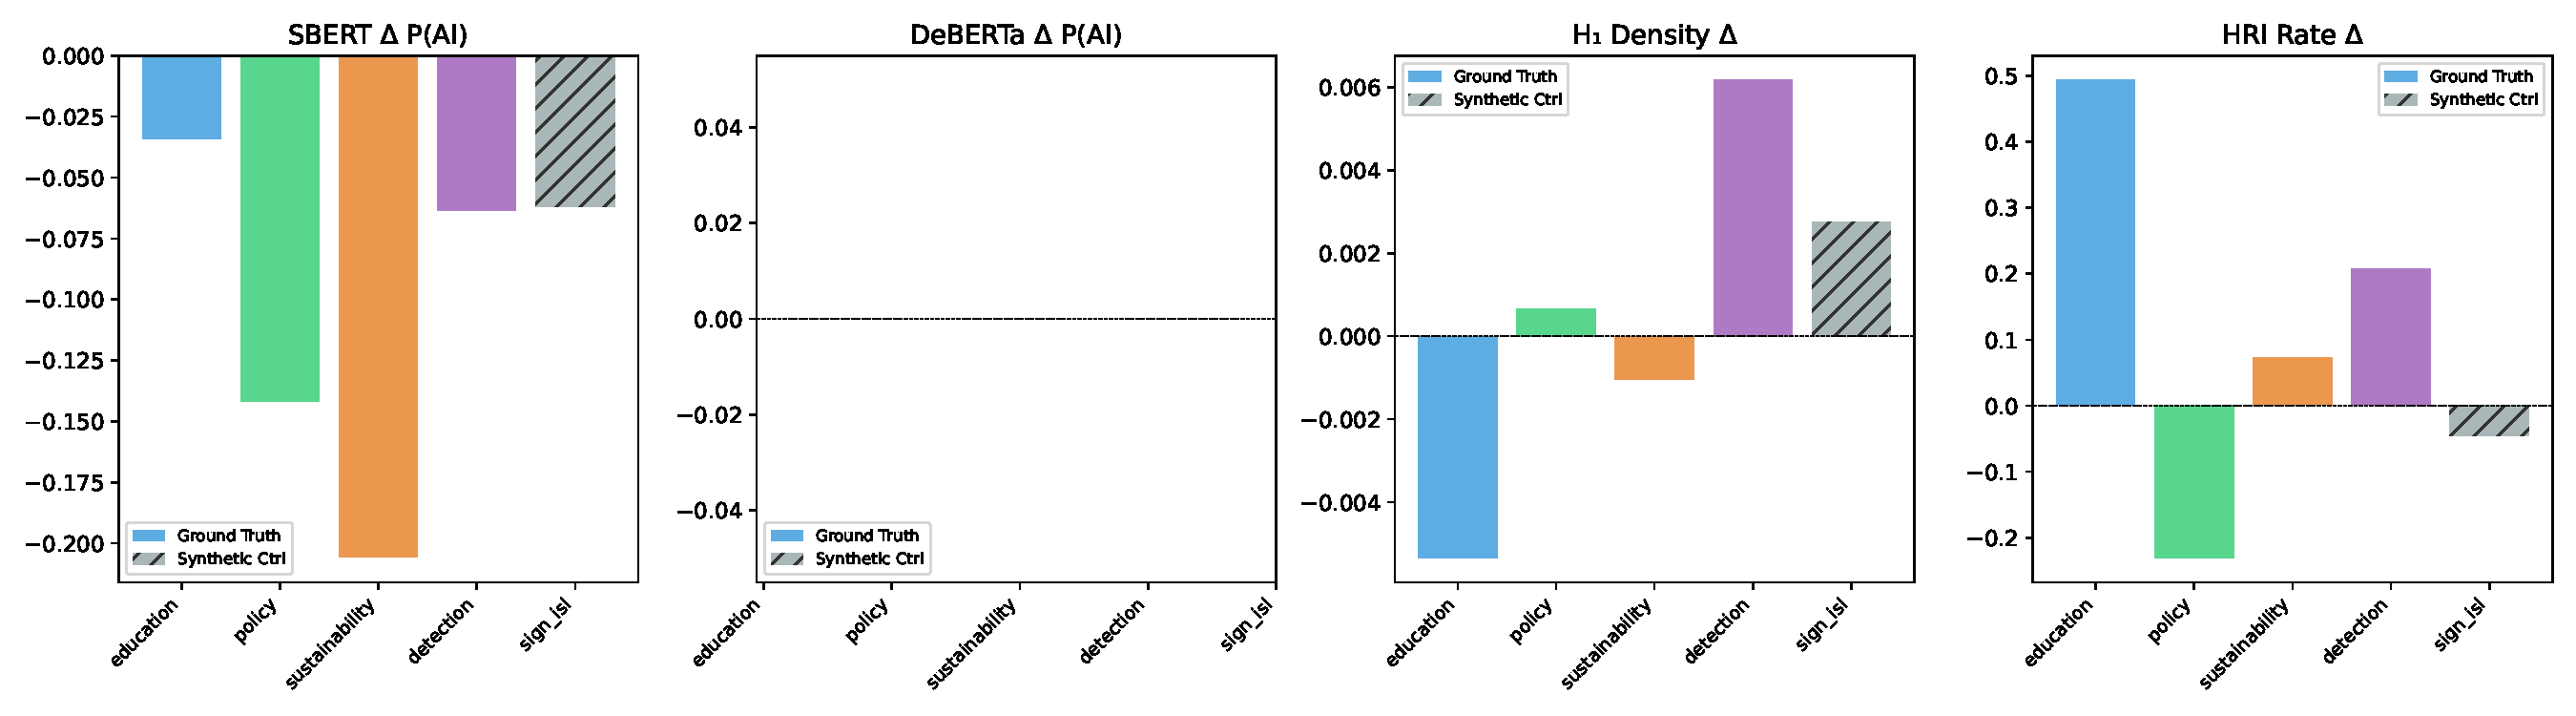
\includegraphics[width=\linewidth]{hrs_metric_deltas.pdf}
    \caption{Metric deltas across HRS pairs.}
    \label{fig:deltas}
\end{figure}

\subsection{Statistical Tests}

\begin{table}[t]
\centering
\small
\caption{Permutation tests ($N = 3$ high-intervention pairs).}
\label{tab:perm}
\begin{tabular}{@{}lccc@{}}
\toprule
\textbf{Metric} & \textbf{Mean$\Delta$} & $p$ & $d$ \\
\midrule
$H_1$ Density   & $+.0001$ & $.433$ & $+0.02$ \\
HRI Rate        & $+.136$  & $.235$ & $+0.45$ \\
SBERT P(AI)     & $-.111$  & $.940$ & $-1.43$ \\
Intra-doc Sim.  & $+.056$  & $.060$ & $+2.27$ \\
\bottomrule
\end{tabular}
\end{table}

$H_1$ density is non-significant ($p = 0.433$, $d = 0.02$). Intra-document similarity shows a large effect ($d = 2.27$, $p = 0.060$) but does not reach significance at $\alpha = 0.05$.

\begin{figure}[t]
    \centering
    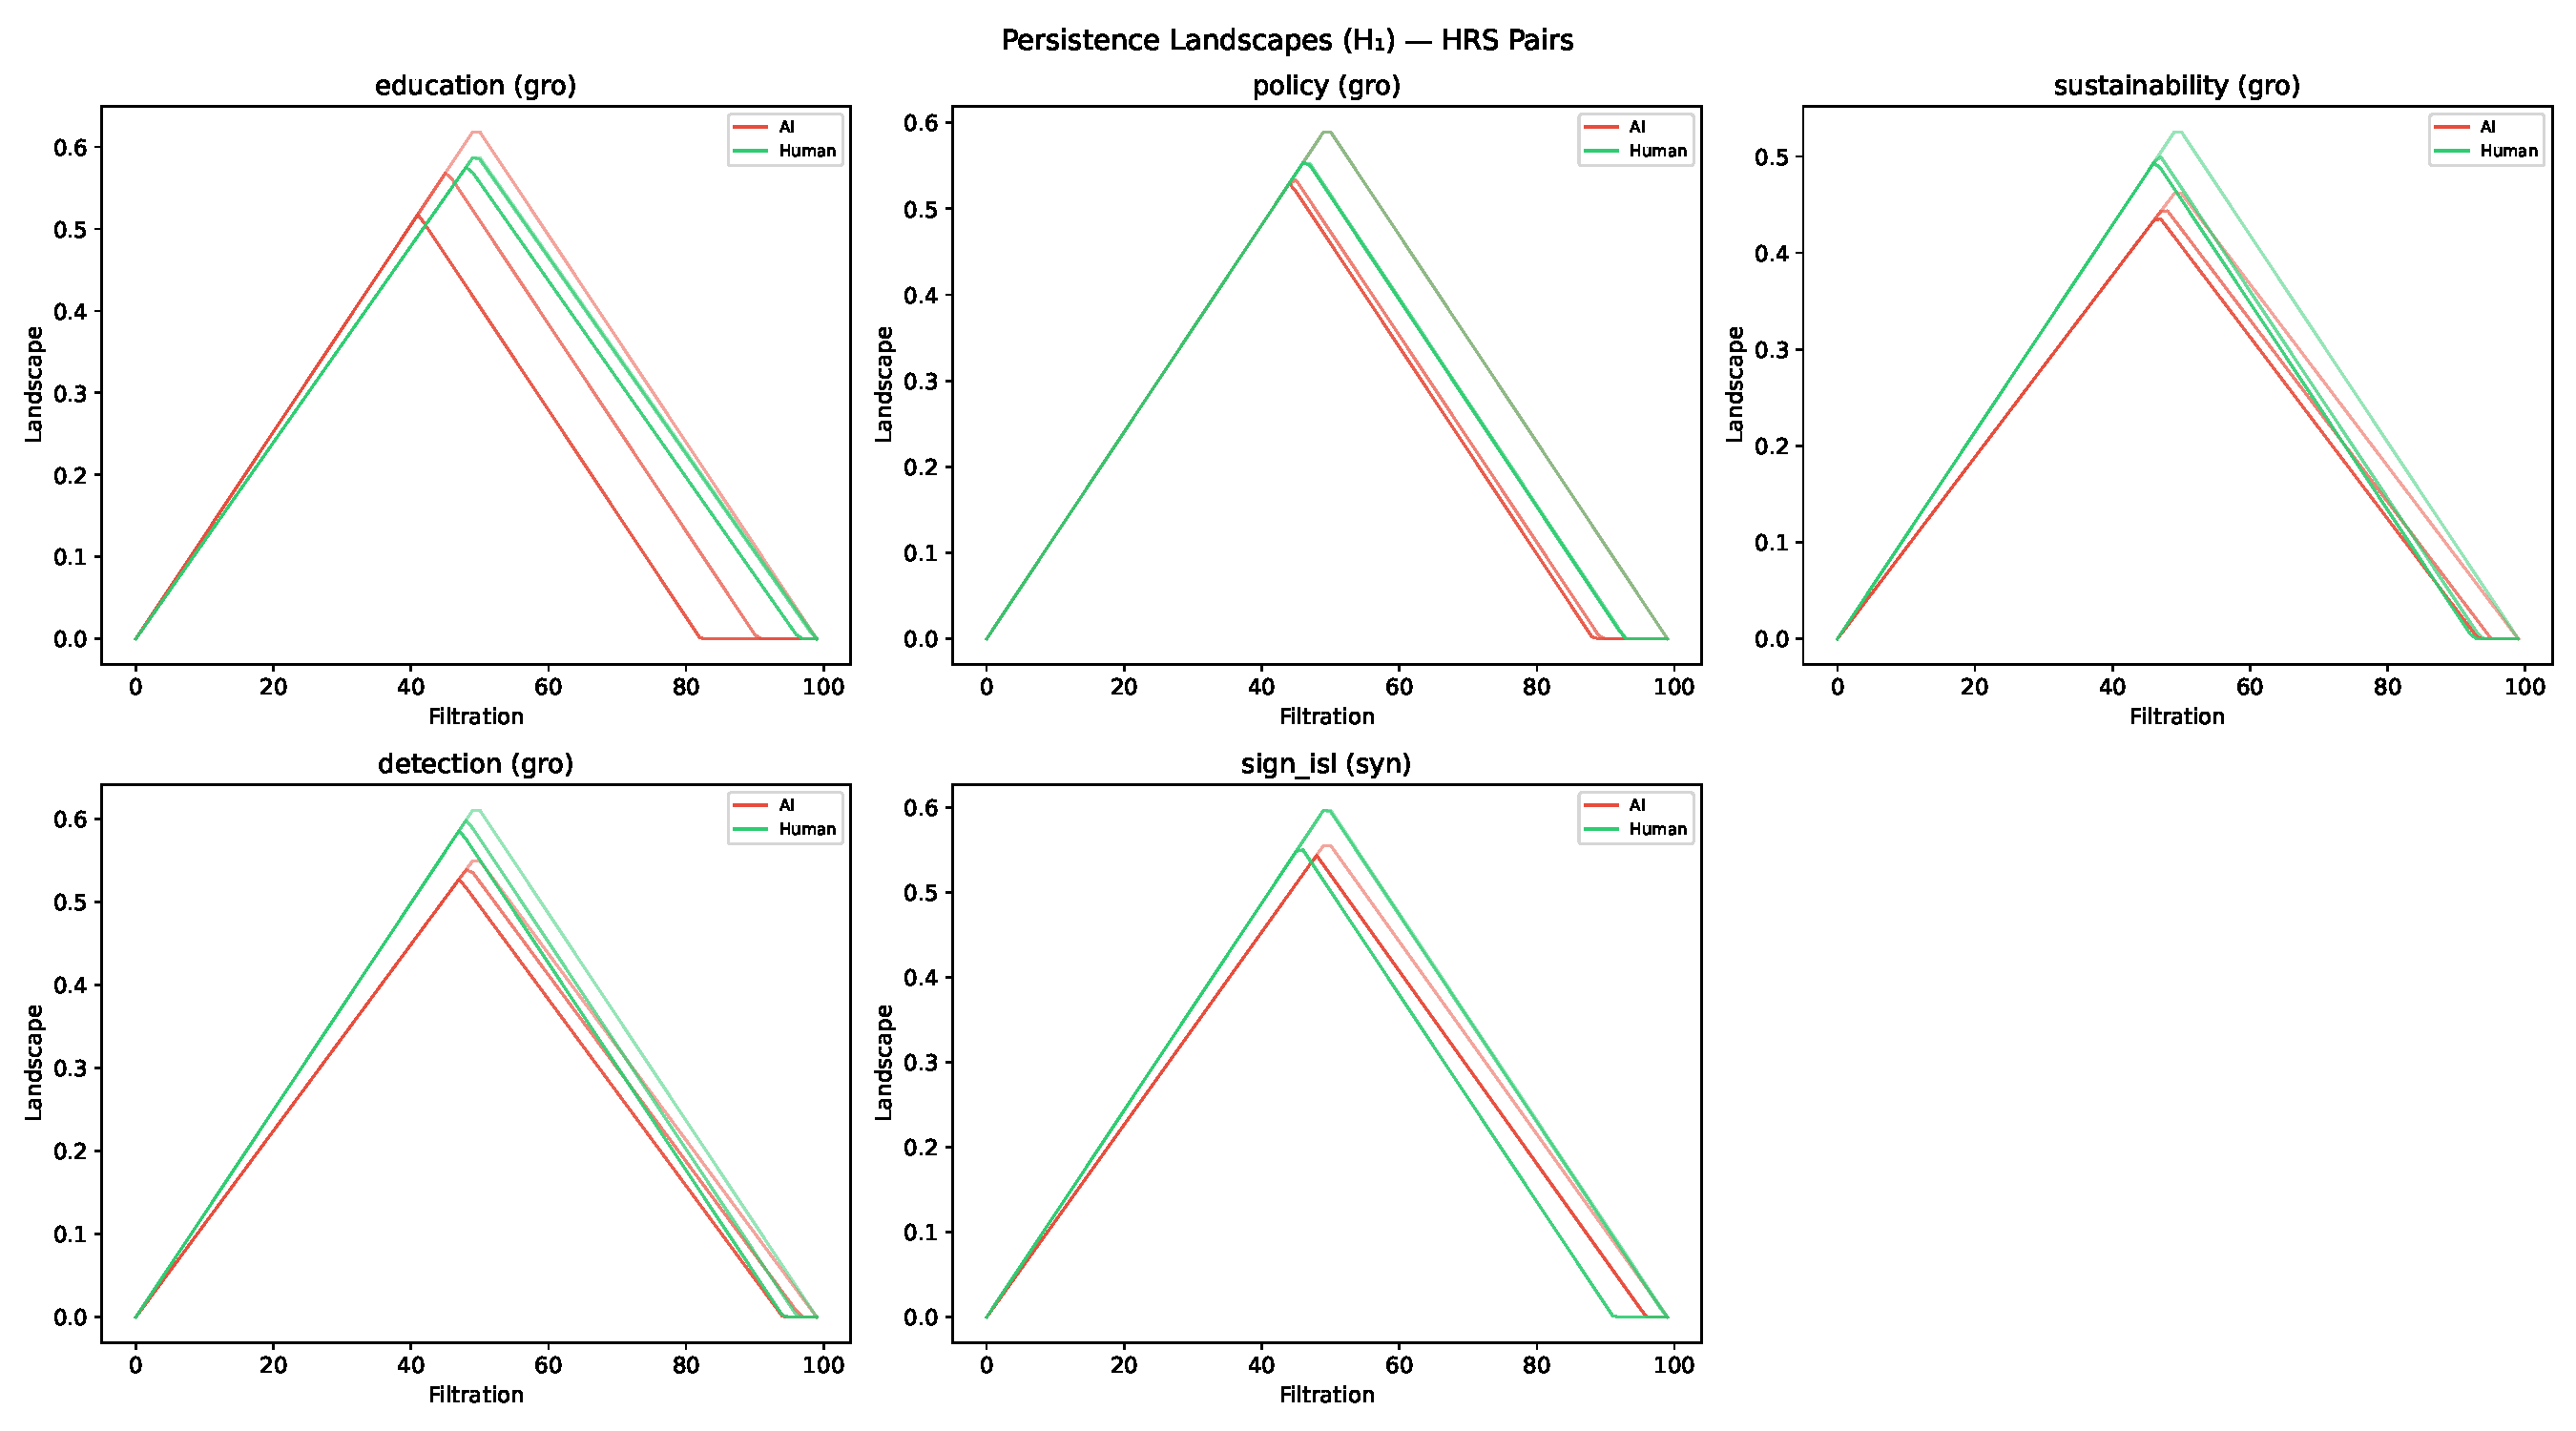
\includegraphics[width=\linewidth]{persistence_landscapes_hrs.pdf}
    \caption{$H_1$ persistence landscapes for HRS pairs.}
    \label{fig:persistence}
\end{figure}

\begin{figure}[t]
    \centering
    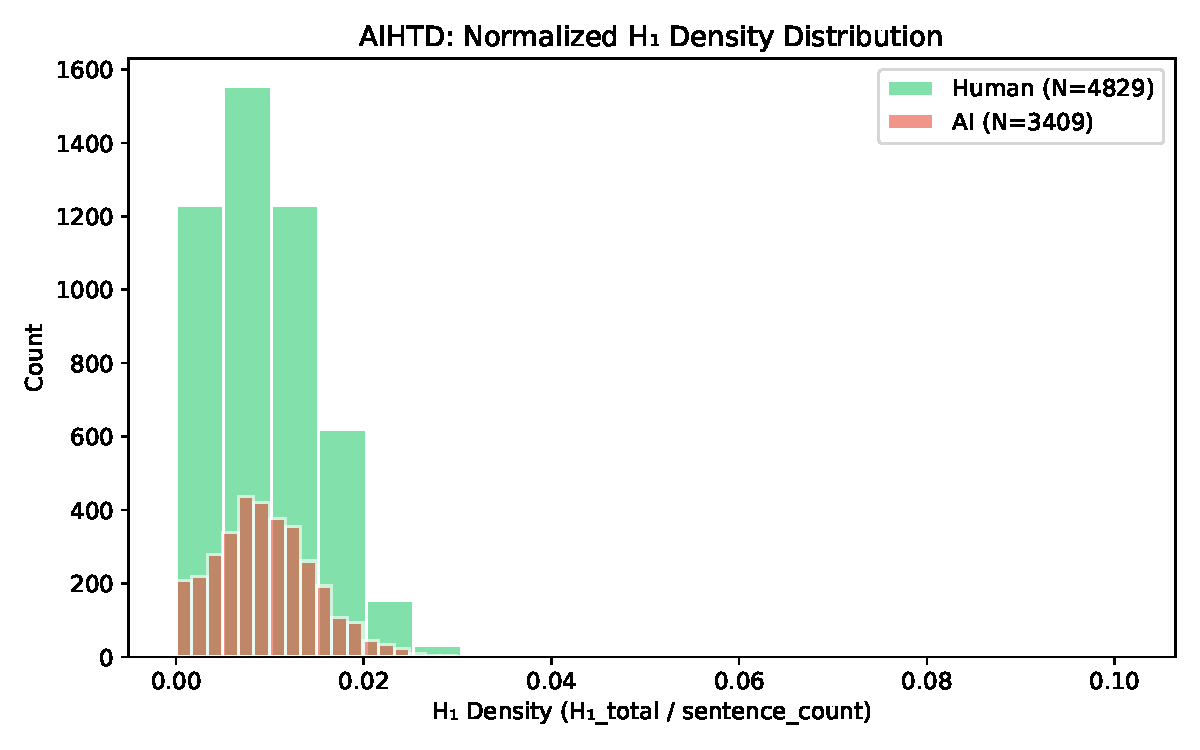
\includegraphics[width=\linewidth]{h1_density_comparison.pdf}
    \caption{$H_1$ density comparison (non-significant).}
    \label{fig:h1}
\end{figure}

\begin{figure}[t]
    \centering
    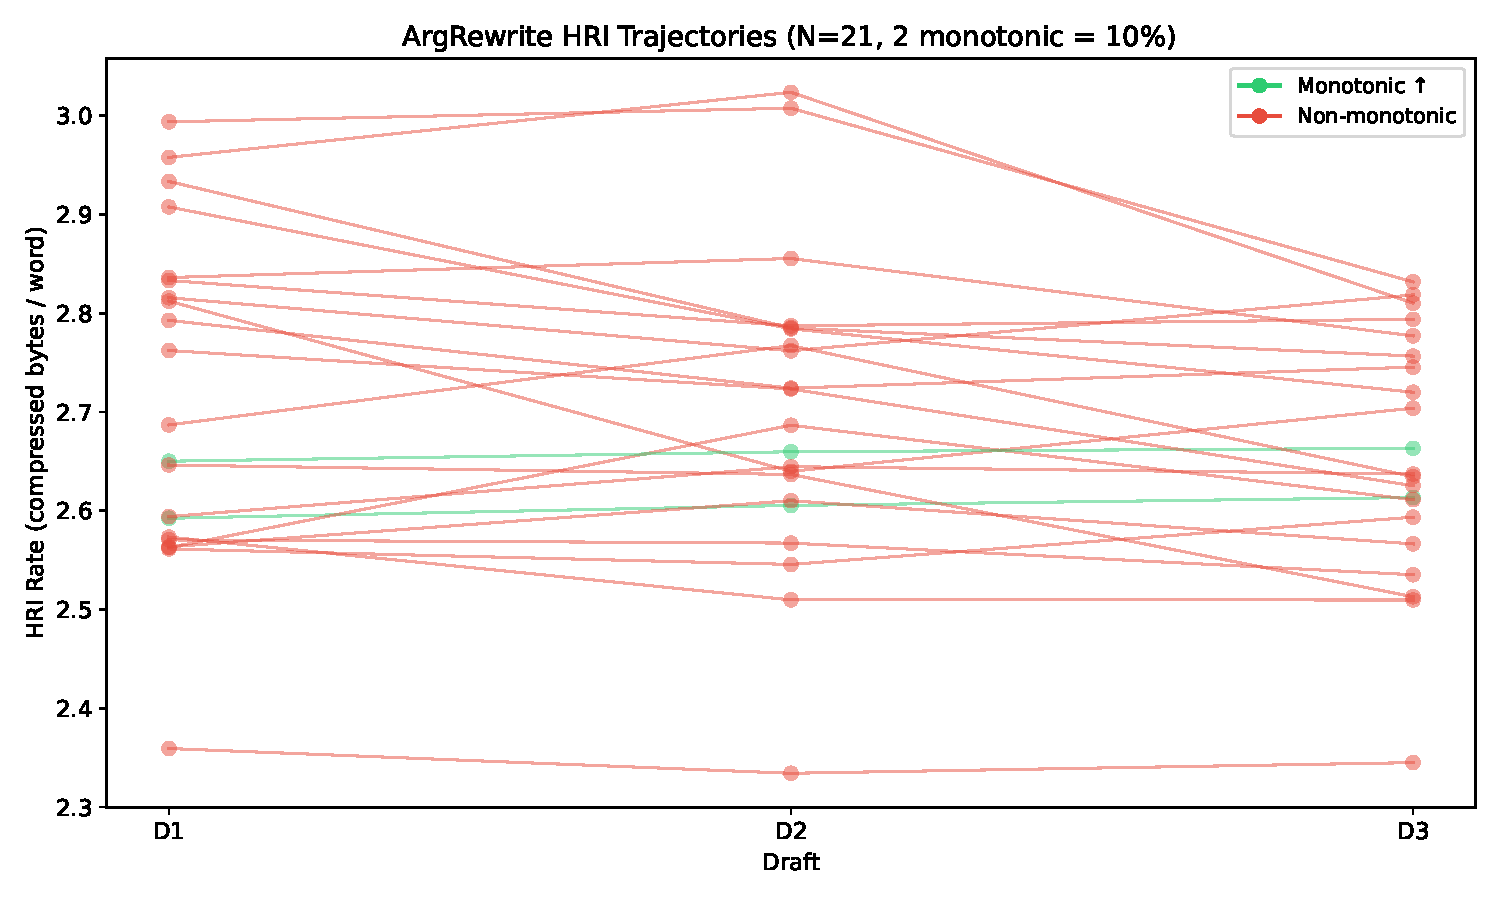
\includegraphics[width=\linewidth]{argrewrite_trajectories.pdf}
    \caption{ArgRewrite HRI trajectories ($N = 21$). Monotonic increase in 61.9\% of essays.}
    \label{fig:argrewrite}
\end{figure}

\section{Discussion}

The consistent response across all three high-intervention pairs suggests that detectors are sensitive to the degree of human editing applied to AI-generated text. The near-maximal deltas ($\Delta \in [-0.982, -0.906]$) indicate that substantial rewriting shifts texts away from patterns the detector associates with AI generation.

Our topological results ($p = 0.433$) contrast with Tulchinskii et al.'s~\cite{tulchinskii2024intrinsic} robust PHD separation, likely due to our dramatically smaller $N$ and topic-controlled design. We present these as exploratory.

\section{Limitations}

\begin{itemize}
    \item HRS $N = 4$ limits statistical power; findings are pilot evidence.
    \item No adversarial robustness testing against paraphrasing~\cite{krishna2024paraphrasing,sadasivan2023reliable}.
    \item AIHTD generator provenance unknown.
    \item Length variation (324--6{,}199 words) may confound non-normalized metrics.
    \item $H_1$ result is non-significant and should not be interpreted as evidence of topological separation.
\end{itemize}

\section{Conclusion}

We introduced a topic-controlled audit methodology for studying how editing depth affects AI text detector response. A fine-tuned DeBERTa classifier achieves near-maximal separation on all three high-intervention pairs, where heavy human editing of AI-generated text shifts detector scores decisively. The zero-intervention anchor confirms the methodology. We contribute the HRS protocol and audit framework as tools for future evaluation of detector sensitivity to editing depth.

\bibliography{custom}
\bibliographystyle{acl_natbib}

\begin{thebibliography}{15}

\bibitem[\protect\citename{Mitchell et al.}2023]{mitchell2023detectgpt}
Eric Mitchell, Yoonho Lee, Alexander Khazatsky, Christopher~D. Manning, and Chelsea Finn.
\newblock 2023.
\newblock {DetectGPT}: Zero-shot machine-generated text detection using probability curvature.
\newblock In \emph{Proc.\ ICML}.

\bibitem[\protect\citename{Hans et al.}2024]{hans2024binoculars}
Abhimanyu Hans, Avi Schwarzschild, Valeriia Cherepanova, Hamid Kazemi, Aniruddha Saha, Micah Goldblum, Jonas Geiping, and Tom Goldstein.
\newblock 2024.
\newblock Spotting {LLMs} with {Binoculars}: Zero-shot detection of machine-generated text.
\newblock In \emph{Proc.\ ICML}.

\bibitem[\protect\citename{Sadasivan et al.}2024]{sadasivan2023reliable}
Vinu~Sankar Sadasivan, Aounon Kumar, Sriram Balasubramanian, Wenxiao Wang, and Soheil Feizi.
\newblock 2024.
\newblock Can {AI}-generated text be reliably detected?
\newblock \emph{JMLR}.

\bibitem[\protect\citename{Cheng et al.}2025]{sadasivan2025adversarial}
Yize Cheng, Vinu~Sankar Sadasivan, Mehrdad Saberi, Shoumik Saha, and Soheil Feizi.
\newblock 2025.
\newblock Adversarial paraphrasing: A universal attack for humanizing {AI}-generated text.
\newblock \emph{arXiv:2412.14637}.

\bibitem[\protect\citename{Wang et al.}2024]{wang2024m4}
Yuxia Wang, Jonibek Mansurov, Petar Ivanov, et~al.
\newblock 2024.
\newblock {M4}: Multi-generator, multi-domain, and multi-lingual black-box machine-generated text detection.
\newblock In \emph{Proc.\ ACL}.

\bibitem[\protect\citename{Krishna et al.}2024]{krishna2024paraphrasing}
Kalpesh Krishna, Yixiao Song, Marzena Karpinska, John Wieting, and Mohit Iyyer.
\newblock 2024.
\newblock Paraphrasing evades detectors of {AI}-generated text, but retrieval is an effective defense.
\newblock In \emph{Proc.\ NeurIPS}.

\bibitem[\protect\citename{Tulchinskii et al.}2024]{tulchinskii2024intrinsic}
Eduard Tulchinskii, Kristian Kuznetsov, Laida Kushnareva, et~al.
\newblock 2024.
\newblock Intrinsic dimension estimation for robust detection of {AI}-generated texts.
\newblock In \emph{Proc.\ NeurIPS}.

\bibitem[\protect\citename{Kushnareva et al.}2023]{kushnareva2023artificial}
Laida Kushnareva, Daniil Cherniavskii, Vladislav Mikhailov, et~al.
\newblock 2023.
\newblock Artificial text detection via examining the topology of attention maps.
\newblock In \emph{Proc.\ EMNLP}.

\bibitem[\protect\citename{Wei et al.}2025]{wei2025shortphd}
Dongjun Wei, Minjia Mao, Xiao Fang, and Michael Chau.
\newblock 2025.
\newblock {Short-PHD}: Detecting short {LLM}-generated text with TDA after off-topic content insertion.
\newblock \emph{arXiv:2504.02873}.

\bibitem[\protect\citename{Mao et al.}2024]{mao2024raidar}
Chengzhi Mao, Carl Vondrick, Hao Wang, and Junfeng Yang.
\newblock 2024.
\newblock {RAIDAR}: Generative {AI} detection via rewriting.
\newblock In \emph{Proc.\ ICLR}.

\bibitem[\protect\citename{Sengupta et al.}2025]{sengupta2025mixrevdetect}
Sandeep Kumar, Samarth Garg, Sagnik Sengupta, Tirthankar Ghosal, and Asif Ekbal.
\newblock 2025.
\newblock {MixRevDetect}: Towards detecting {AI}-generated content in hybrid peer reviews.
\newblock In \emph{Proc.\ NAACL}.

\bibitem[\protect\citename{He et al.}2023]{he2021debertav3}
Pengcheng He, Jianfeng Gao, and Weizhu Chen.
\newblock 2023.
\newblock {DeBERTaV3}: Improving {DeBERTa} using {ELECTRA}-style pre-training.
\newblock In \emph{Proc.\ ICLR}.

\bibitem[\protect\citename{Reimers and Gurevych}2019]{reimers2019sentencebert}
Nils Reimers and Iryna Gurevych.
\newblock 2019.
\newblock {Sentence-BERT}: Sentence embeddings using {S}iamese {BERT}-networks.
\newblock In \emph{Proc.\ EMNLP}.

\bibitem[\protect\citename{Gehrmann et al.}2019]{gehrmann2019gltr}
Sebastian Gehrmann, Hendrik Strobelt, and Alexander~M. Rush.
\newblock 2019.
\newblock {GLTR}: Statistical detection and visualization of generated text.
\newblock In \emph{Proc.\ ACL}.

\bibitem[\protect\citename{Yang et al.}2023]{yang2023dnagpt}
Xianjun Yang, Wei Cheng, Yue Wu, Linda Petzold, William~Yang Wang, and Haifeng Chen.
\newblock 2023.
\newblock {DNA-GPT}: Divergent n-gram analysis for training-free detection of {GPT}-generated text.
\newblock \emph{arXiv:2305.17359}.

\end{thebibliography}

\end{document}
